\chapter{برنامجك الأوّل}

لقد قمنا بحضير كلّ شيء إلى حد الآن ويمكننا أن نبدأ قليلا من البرمجة. مع نهاية هذا الفصل ستكون قد نجحت في إنشاء أوّل برنامج لك.

لكي أصدقك القول، سيظهر البرنامج بالأبيض والأسود ولن يقوم بشيء سوى إلقاء التحيّة. يبدو عديم الفائدة، لكنّه برنامجك الأوّل وأؤكّد لك أنّك ستكون فخورا به.

\section{كونسول أو نافذة ؟}

لقد تحدثنا سابقا عن فكرة برامج الكونسول وبرامج النوافذ في الفصل السابق. البيئة التطويرية تطلب منا تحديد أي نوع من البرامج نريد أن ننشئها. ولقد قلنا إننا سننشئ برامج من نوع كونسول.

يوجد نوعان من البرامج، لا أكثر :

\begin{itemize}
  \item ،برامج بنوافذ
  \item برامج تعمل في الكونسول.
\end{itemize}

\subsection{البرامج الّتي تملك نوافذ}

هي البرامج التي نعرفها جميعا. هذا مثال على برنامج من نوع نافذة، مثل الرسام.

\begin{figure}[H]
	\centering
	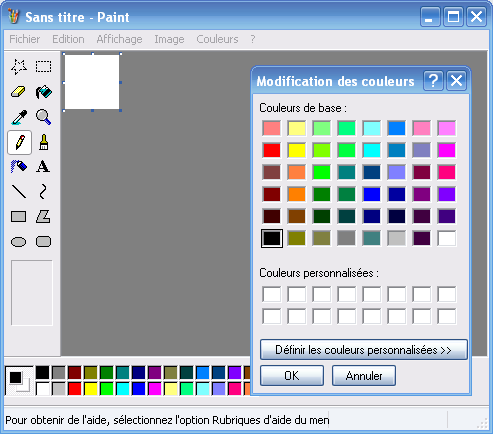
\includegraphics[width=0.8\textwidth]{Chapter_I-3_Paint}
\end{figure}

أعتقد أنّك تحب إنشاء برامج كهذه، لكنّ هذا ليس في مقدورك حاليا. في الواقع، إنشاء برامج بنوافذ هو أمر ممكن بلغة \textenglish{C}، لكنّ بالنسبة لمبتدئ، هذا أمر معقّد جدّا. كبداية، يستحسن إنشاء برامج الكونسول.

\begin{question}
  لكن ماذا يعنى برنامج
\textenglish{Console}
؟
\end{question}

\subsection{البرامج الّتي تعمل في الكونسول}

برامج الكونسول هي أول ما ظهر من برامج. في ذلك الوقت، شاشات الحواسيب لم تكن سوى بالأبيض والأسود، ولم تكن فعّالة لكي تتمكّن من رسم النوافذ كما هو الحال مع حواسيبنا حاليّا.

مرّ الزمن بسرعة وزادت شعبية الويندوز نظراً لبساطته إلى أن نسي كثير من الناس ما هي الكونسول.

لديّ خبر جيّد لك !
\textbf{الكونسول لم تمت بعد} !
 في الواقع،
\textenglish{GNU/Linux}
 قد أعاد الكونسول إلى الحياة. هذه صورة لكونسول على
\textenglish{GNU/Linux}.

\begin{figure}[H]
	\centering
	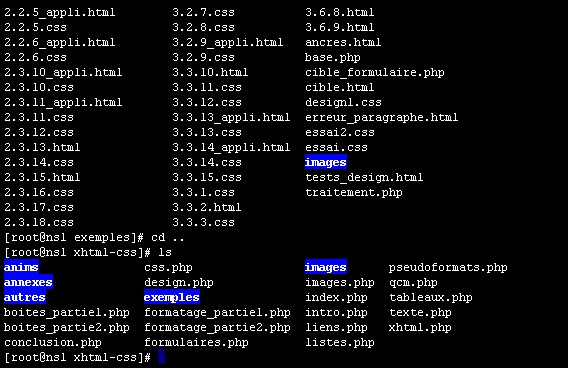
\includegraphics[width=0.9\textwidth]{Chapter_I-3_Console}
\end{figure}

مرعب ! صحيح ؟ لكن على الأقل عرفت ما هي الكونسول، وهذه بعض الملاحظات :

\begin{itemize}
  \item اليوم، يمكننا عرض الألوان في الكونسول. ليس كلّ شيء بالأبيض والأسود كما تتخيّل.
  \item الكونسول هو الأسهل من ناحية البرمجة بالنسبة للمبتدئين.
  \item أداة عالية الإمكانيّات إذا عرفنا كيف نستخدمه.
\end{itemize}

كما قلت لك، إنشاء برامج كونسول أمر سهل جدّا وملائم للمبتدئين (وهذا عكس برامج النوافذ). ليكن في علمك أيضا أنّ الكونسول قد تطوّرت وبإمكانها عرض الألوان، ولا شيء يمنعك من إضافة صورة خلفيّة لها.

\begin{question}
  وفي الويندوز ألا توجد
\textenglish{Console}
 ؟
\end{question}

بلى، لكنّها مخفيّة لو صح القول. يمكنك فتحها بالذهاب إلى "إبدأ"
(\InlineCode{Start})
 ثمّ "ملحقات"
(\InlineCode{Accessories})
 ثمّ "موجه الأوامر"
(\InlineCode{Command prompt})
 أو بالذهاب إلى "إبدأ" ثمّ "تشغيل"
(\InlineCode{Run})
 واكتب فيها
\InlineCode{cmd}
 واضغط على "موافق".

\begin{figure}[H]
	\centering
	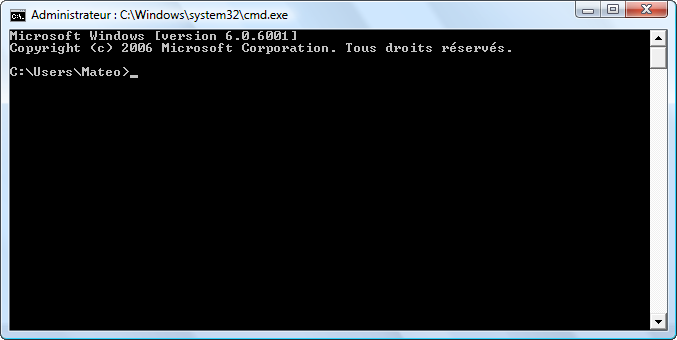
\includegraphics[width=0.8\textwidth]{Chapter_I-3_Console-Windows}
\end{figure}

إذا كنت تستخدم نظام ويندوز، فاعلم بأن أولى برامجك ستكون في نوافذ شبيهة بهذه. أنا لم أختر البداية هكذا لجعلك تشعر بالملل، بل لتعليمك الأساسيّات اللازمة لكي تتمكّن لاحقا من إنشاء النوافذ.

إذن فلتكن متيقّناً، بمجرّد أن تصل إلى المستوى اللازم لإنشاء النوافذ، سوف أعلّمك كيف تفعل ذلك.

\section{الحدّ الأدنى من الشفرة المصدرية}

من أجل أي برنامج، يجب كتابة قدر معيّن من الشفرة المصدرية. هذه الشفرة لا تقوم بشيء خاصّ لكنّها ضروريّة. هذه الشفرة التي سنكتشفها الآن ستكون أساس أغلب برامجك الّتي ستكتبها بلغة \textenglish{C}.

\subsection{أطلب من البيئة التطويرية الخاصة بك تزويدك بالحد الأدنى من الشفرة المصدرية}

لقد لاحظت أن طريقة إنشاء مشروع جديد تختلف من بيئة تطويرية إلى أخرى. إليك تذكيراً بسيطا : في برنامج
\textenglish{Code::Blocks}
 (الذي سنستخدمه في هذا الكتاب)، عليك التوجه نحو
\InlineCode{File}
 ثمّ
\InlineCode{New}
 ثمّ
\InlineCode{Project}
 ثم تختار
\InlineCode{Console Application}
 وبعدها اللغة
\textenglish{C}.
سيولّد لك الحد الأدنى من الشفرة المصدرية
 \textenglish{C}
 التي تحتاجها. ها هي :

\begin{Csource}
#include <stdio.h>
#include <stdlib.h>

int main()
{
    printf("Hello world!\n");
    return 0;
}

\end{Csource}

\begin{information}
لاحظ أنّه يوجد سطر فارغ في نهاية الشفرة. يفترض أن ينتهي كل ملف مكتوب بلغة
\textenglish{C}
هكذا. إن لم تفعل ذلك، فهذه ليست بمشكلة، لكن توقّع أن يعرض لك المترجم تحذيراً
(\textenglish{Warning}).
\end{information}

علماً أنّ السطر :
\begin{Csource}
int main()
\end{Csource}
\dots
بإمكانه أن يُكتب كالتالي :

\begin{Csource}
int main(int argc, char *argv[])
\end{Csource}

كلتا العبارتين تحملان نفس المعنى لكن الثانية، الأكثر تعقيدا، هي الأكثر شيوعا، لذلك فإنّنا سنستخدمها في الفصول القادمة.\\
إستخدامنا للشكل الأوّل أو الثاني لا يغيّر شيئا بالنسبة لنا. لذلك لا داعي لإضاعة الوقت هنا، خصوصاً أنّك لا تملك المستوى اللازم لفهم ما تعنيه.

إذا كنت تستخدم بيئة تطويرية أخرى فقم بنسخ هذه الشفرة المصدرية وألصقها في الملف \InlineCode{main.c} ليكون لديكم نفس الشفرة.

أخيرا، قم بحفظ عملك في المشروع. أعلم أننا لم نقم بشيء حتّى الآن لكن من الجيّد التعوّد على الحفظ في كلّ مرّة.

\subsection{تحليل أسطر الشفرة المصدرية السابقة}
قد تبدو لك الشفرة المصدرية السابقة أنّها كاللغة الصينيّة، أنا أتخيّل ذلك ! في الواقع هي تسمح بإنشاء برنامج كونسول يعرض نصّا على الشاشة. يجب تعلّم كيفيّة قراءة كلّ هذا.

فلنبدأ بأوّل سطرين :
\begin{Csource}
#include <stdio.h>
#include <stdlib.h>
\end{Csource}

هذان السطران يبدآن بعلامة
\InlineCode{\#}.
وهي أسطر خاصّة تُعرف باسم
\textbf{توجيهات المعالج القبلي}
(\textenglish{Preprocessor directives})
. اسم معقّد، أليس كذلك ؟ هذه الأسطر تتمّ قراءتها من طرف البرنامج المسمّى بالمعالج القبلي، وهو برنامج يتمّ تشغيله في بداية الترجمة.

ما رأيناه سابقا كان مخطّطا بسيطا لعمليّة الترجمة. لكنّ في الواقع، هناك الكثير من المراحل التي تحدث في هذه العمليّة. سنقوم بتفصيل هذا لاحقا. حاليّا عليك فقط تذكّر وضع هذين السطرين أعلى كلّ ملفّاتك.

\begin{question}
  حسنا لكن ماذا يعنيه هذان السطران ؟ أريد أن أعرف !
\end{question}

كلمة
 \InlineCode{include}
 بالإنجليزيّة تعني "تضمين". هذان السطران يقومان بتضمين ملفّات في المشروع، أي إضافة هذه الملفّات من أجل عمليّة الترجمة. هناك سطران وبالتالي هناك ملفان يتمّ تضمينهما في المشروع وهما بالترتيب :
\InlineCode{stdio.h}
 و
\InlineCode{stdlib.h}.
هذان الملفّان موجودان بالفعل على حاسوبك وهما ملفّان مصدريّان جاهزان، سوف تعرف مستقبلا أنّنا نسميها
\textbf{مكتبات}
(\textenglish{Libraries}).
 هذه الملفّات تحتوي الشفرة المصدرية اللازمة لعرض نصّ على الشاشة.

 بدون هذين الملفّين، كتابة نصّ على الشاشة سيكون أمرا مستحيلاً. فالحاسوب لا يعرف فعل أي شيء مبدئيا.

 باختصار، السطران الأول والثاني يقومان بتضمين المكتبات التي ستساعدنا في إظهار نصّ على الشاشة بكلّ سهولة.

 نمر للتالي، باقي الأسطر :
 
\begin{Csource}
int main()
{
    printf("Hello world!\n");
    return 0;
}
\end{Csource}

ما تراه هنا هو ما نسميه بـ\textbf{التابع}
أو
\textbf{الدالّة}
(\textenglish{Function}).
 البرنامج في لغة
\textenglish{C}
 يتكوّن من مجموعة دوال. حاليّا برنامجنا لا يحوي سوى دالّة واحدة.

الدالّة تمكّننا من تجميع مجموعة من الأوامر. الغرض من تجميع الأوامر هو جعلها تقوم بوظيفة ما. مثلا يمكننا إنشاء دالّة باسم
 \InlineCode{open\_file}
 وجعلها تحتوي التعليمات التي تشرح للحاسوب كيفيّة فتح ملف.

 دون الدخول في تفاصيل إنشاء الدالّة (الوقت مبكّر، سوف نتحدّث عن الدوال في وقت لاحق) لنحلّل رغم ذلك أجزائه الكبيرة. السطر الأوّل يحتوي اسم الدالّة، إنّه الكلمة الثانية.\\
 أجل، اسم دالّتنا هو
\InlineCode{main}
والذي يعني
"الرئيسية"
. وتشغيل البرنامج دائما يبدأ من الدالة
\InlineCode{main}.

للدالّة بداية ونهاية، وهي محدودة بالحاضنتين
\InlineCode{\{}
و
\InlineCode{\}}.
محتوى الدالّة موجود بين هاتين الحاضنتين. إن كنت قد تابعت جيداً فقد عرفت أنّ الدالّة مشكّلة من سطرين :

\begin{Csource}
printf("Hello world!\n");
return 0;
\end{Csource}

هاته الأسطر في الداخل نسميها
\textbf{التعليمات}
(\textenglish{Instructions})
 (هذه إحدى المصطلحات الّتي يجب عليك حفظها). كلّ تعليمة تمثّل أمراً بالنسبة للحاسوب. فكلّ واحدة منها تطلب منه فعل شيء محدّد.

 كما قلت لك، بتجميع ذكيّ للتعليمات في الدالّة يمكننا إنشاء أجزاء برنامج جاهزة للاستخدام. باستخدام التعليمات المناسبة يمكننا إنشاء دالّة
 \InlineCode{open\_file}
 كما شرحت لك قبل قليل، و أيضا دالّة
\InlineCode{move\_character}
 في لعبة فيديو، على سبيل المثال.

 البرنامج في الواقع ما هو إلّا تتابع لتعليمات : إفعل هذا و إفعل ذاك. أنت تعطي أوامر للحاسوب و هو يقوم بتنفيذها.

 \begin{critical}
هامّ جدّا : لا بدّ أن تنتهي كلّ تعليمة بفاصلة منقوطة
"\InlineCode{;}"
. بهذا يمكن التفريق بين ما إذا كانت هذه تعليمة أم لا. إذا نسيت وضع فاصلة منقوطة نهاية تعليمة ما، فلن تتمّ ترجمة برنامجك.
 \end{critical}

 السطر الأول :
 \InlineCode{printf("Hello world!\\n");}
 يطلب إظهار الرسالة
 "\textenglish{Hello world!}"
  على الشاشة. عندما يصل برنامجك إلى هذا السطر، فسوف يقوم بعرض هذه الرسالة ثمّ المرور إلى التعليمة التالية.

  التعليمة التالية هي
\InlineCode{return 0;}
 و هي تخبرنا أنّ الدالّة
\InlineCode{main}
 قد انتهت و تطلب منه إعادة 0.

 \begin{question}
   لماذا يقوم برنامجي بإعادة العدد 0 ؟
 \end{question}

 في الواقع، كلّ برنامج عندما ينتهي يُرجع قيمة معينة. على سبيل المثال، ليقول أنّ كلّ شيء سار على ما يرام. عمليّا، 0 يعني  أنّ كلّ شيء سار على ما يرام، و كلّ قيمة أخرى تدلّ على حدوث خطأ. في أغلب الأحيان هذه القيمة لا تُستخدم ، لكن يجب رغم ذلك استعمالها.\\
 كان يمكن أن يعمل برنامجك بدون
 \InlineCode{return 0}
، لكن يمكننا القول أن وضعها يعتبر أمراً أكثر نظافة و أكثر جدّية.

إلى هنا نكون قد فصّلنا قليلا في عمل هذه الشفرة المصدرية.

طبعا، نحن لم ندرس كلّ شيء بعمق، و قد تكون لديك بعض الأسئلة عالقة في ذهنك. كن على يقين بأنك ستجد لها أجوبة شيئا فشيئا مع تقدّمنا في الكتاب. لا يمكنني أن أطلعك على كلّ شيء من البداية، لأنّ هناك كثيراً من الأشياء لاستيعابها.

إليك ما يلي : بما أنني في حال جيّدة، سأقوم بوضع مخطّط يضمّ المصطلحات الّتي تعلّمناها في هذا الفصل.

\begin{figure}[H]
	\centering
	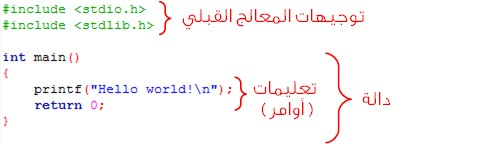
\includegraphics[width=0.8\textwidth]{Chapter_I-3_HelloWorld}
\end{figure}

\subsection{لنجرّب برنامجنا}

كلّ ما سنقوم به الآن هو ترجمة المشروع ثمّ تشغيله (اضغط على
\InlineCode{Build \& Run}
 إذا كنت على
\textenglish{Code::Blocks}).
سيطلب منك حفظ مشروعك إذا لم تقم بذلك من قبل.

\begin{critical}
  إن لم تنجح الترجمة و ظهر لك خطأ مثل :\\
\InlineCode{"My-program - Release" uses an invalid compiler. Skipping...}\\\InlineCode{Nothing to be done...}
فهذا يعني أنّك نزلت نسخة
\textenglish{Code::Blocks}
 دون
\InlineCode{mingw}
 (المترجم)، عد و نزّل النسخة التي تحتوي على
\InlineCode{mingw}.
\end{critical}

بعد بُرهة، يظهر برنامجك كما في الصورة :

\begin{figure}[H]
	\centering
	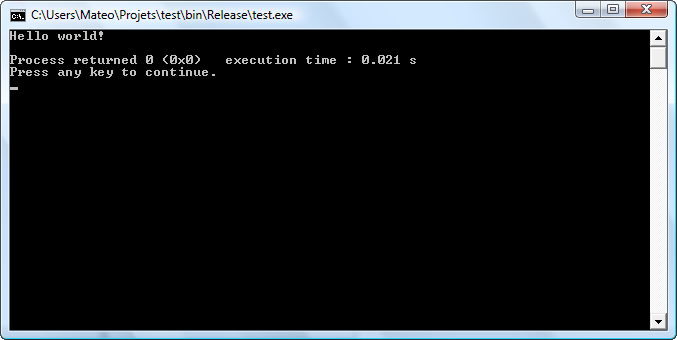
\includegraphics[width=0.9\textwidth]{Chapter_I-3_HelloWorld-run}
\end{figure}

البرنامج يُظهر
"\textenglish{Hello world!}"
 (في السطر الأوّل).\\
الأسطر الّتي أسفله تمّ توليدها من طرف
\textenglish{Code::Blocks}
 وتدلّ على أنّ البرنامج قد تمّ تشغيله بنجاح كما أنها تعطي الوقت الذي استغرقه البرنامج في التشغيل.

 سيطلب منك الضغط على إحدى المفاتيح لإغلاق النافذة. أعلم أن الأمر لم يكن ممتعا جدّا. لكنه برنامجك الأوّل، وهذه لحظة ستتذكرها طيلة حياتك ! ألا تعتقد ذلك ؟

\section{كتابة رسالة على الشاشة}

من الآن سنقوم بإدخال التعديلات على الشفرة المصدرية السابقة. مهمّتك، إن قبلتها : عرض رسالة
"\textenglish{Bonjour}"
 على الشاشة.

\begin{question}
  كيف يمكنني اختيار النص الّذي سيظهر على الشاشة ؟
\end{question}

الأمر بسيط جدا، إذا بدأت من الشفرة التي رأيناها سابقاً، فسيكون عليك استبدال
"\textenglish{Hello world!}"
 بـ"\textenglish{Bonjour}"
 في السطر الذي يستدعي
\InlineCode{printf}.

كما قلت من قبل،
\InlineCode{printf}
 هي
\textbf{تعليمة}
 وهي تعطي أمراً للحاسوب : "قم بعرض هذه الرسالة على الشاشة".\\
يجب أن تعرف أيضا أن
\InlineCode{printf}
 هي دالّة كُتِبَت من قبل من طرف مبرمجين قبلك.

\begin{question}
   أين توجد هذه الدالّة ؟ أنا لا أرى سوى الدالّة \InlineCode{main} !
\end{question}

هل تذكر هذين السطرين ؟

\begin{Csource}
#include <stdio.h>
#include <stdlib.h>
\end{Csource}

قلت لك من قبل أنهما يمكنان البرنامج من إضافة مكتبات. المكتبات في الحقيقة هي ملفّات تحوي أطنانا من الدوال جاهزة للإستخدام. هذه الملفات
(\InlineCode{stdio.h} و \InlineCode{stdlib.h})
 تحوي أغلب الدوال الأساسية التي قد نحتاجها في برنامج ما.
\InlineCode{stdio.h}
 بحد ذاته يحوي دوال تمكّن من عرض أشياء على الشاشة (مثل
 \InlineCode{printf})
 و أيضا الطلب من المستخدم إدخال شيء ما (هذه دوال سنتعرّف عليها لاحقا).

\subsection{لنقل مرحبا للسيّد}

في دالّتنا
\InlineCode{main}
نستدعي الدالّة
 \InlineCode{printf}.
 أي أن لدينا دالّة تستدعي أخرى (هنا
\InlineCode{main}
تستدعي
\InlineCode{printf}).
سترى أن هذا ما يحدث دائما في لغة
\textenglish{C}
: دالّة تحتوي تعليمات تستدعي دوال أخرى، وهكذا.

إذن، لاستدعاء دالّة يكفي كتابة اسمها متبوعا بقوسين، ثم فاصلة منقوطة.

\begin{Csource}
printf();
\end{Csource}

هذا جيد، لكنه غير كاف. يجب أن نُعلم البرنامج بما يجب أن يكتبه في الشاشة. لفعل هذا يجب أن نعطي
\InlineCode{printf}
النص المطلوب عرضه. لفعل هذا نقوم بوضع النص داخل علامات الإقتباس المزدوجة بين القوسين.\\
في حالتنا هذه سنكتب تماما :

\begin{Csource}
printf("Bonjour");
\end{Csource}

آمل ألا تكون قد نسيت رمز الفاصلة المنقوطة في النهاية، وأذكّرك أنّها مهمّة جدا لأنّها تدلّ على نهاية التعليمة.\\
هذه هي الشفرة المصدرية التي يجب أن تحصل عليها :

\begin{Csource}
#include <stdio.h>
#include <stdlib.h>

int main()
{
    printf("Bonjour");
    return 0;
}
\end{Csource}

لدينا إذن تعليمتان تطلبان من الحاسوب القيام بهذين الأمرين بهذا الترتيب :
\begin{enumerate}
  \item عرض
"\textenglish{Bonjour}"
على الشاشة.
  \item نهاية الدالّة
\InlineCode{main}
، إعادة 0. البرنامج يتوقّف.
\end{enumerate}

هذا ما يظهر على شاشتك :

\begin{figure}[H]
	\centering
	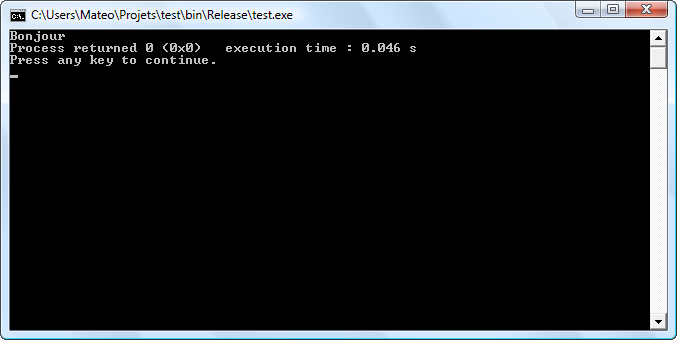
\includegraphics[width=0.9\textwidth]{Chapter_I-3_Good-Morning}
\end{figure}

كما ترى، السطر الذي يحتوي الرسالة يكون ملتصقاً قليلا بباقي النص، على خلاف ما رأيناه سابقا.\\
أحد الحلول الممكنة هو إضافة رمز للعودة إلى السطر بعد
 "\textenglish{Bonjour}"
 (كما لو أنّنا ضغطنا على المفتاح
\InlineCode{Enter}).

ولكن ضغط المفتاح
\InlineCode{Enter}
 في الشفرة المصدرية لن يعمل كما تتوقع، لهذا يجب استخدام المحارف الخاصّة
(\textenglish{Special characters}).

\subsection{المحارف الخاصّة}

المحارف أو الرموز الخاصّة هي محارف تمكّن من تعريف عودة إلى السطر، جدولة، إلخ.\\
من السهل التعرّف عليها، فهي مكوّنة من محرفين. الأوّل هو الشَرْطَةُ المائلة الخلفية 
(\textbackslash) (\textenglish{Backslash})
والثاني يكون رقما أو حرفا. إليك محرفين خاصّين قد تحتاجهما كثيرا :

\begin{itemize}
  \item \InlineCode{\textbackslash n} :
 العودة إلى السطر.
 \item \InlineCode{\textbackslash t} :
 الجدولة (فراغ كبير في نفس السطر).
\end{itemize}

في حالتنا هذه، يكفي أن نكتب
\InlineCode{\textbackslash n}
 لإنشاء العودة إلى السطر. إذن، إذا أردنا أن نضع عودة إلى السطر بعد
\textenglish{Bonjour}
، فيكفي أن نكتب :

\begin{Csource}
printf("Bonjour\n");
\end{Csource}

وسيفهم حاسوبك أنّ عليه كتابة
"\textenglish{Bonjour}"
 ويعود إلى السطر.

\begin{figure}[H]
	\centering
	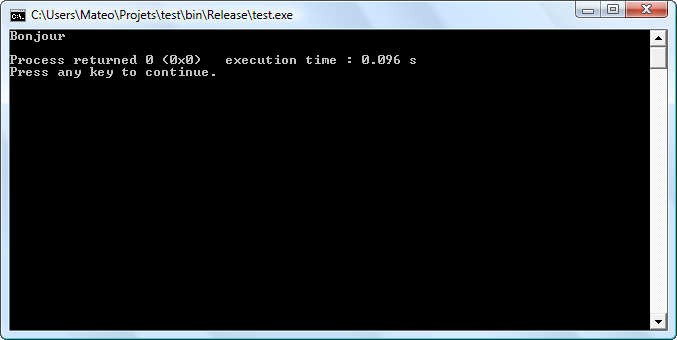
\includegraphics[width=0.9\textwidth]{Chapter_I-3_Good-Morning-backslash-n}
\end{figure}

\begin{information}
  يمكنك الكتابة بعد
\InlineCode{\textbackslash n}
بدون أيّة مشكلة. كلّ ما تكتبه بعد
\InlineCode{\textbackslash n}
 سيوضع في السطر الجديد. يمكنك إذن التدرّب على كتابة :
\InlineCode{printf("Good morning\textbackslash nGood bye\textbackslash n");}\\
و سيتمّ عرض
"\textenglish{Good morning}"
على السطر الأوّل و
"\textenglish{Good bye}"
على السطر الثاني.
\end{information}

\subsection{متلازمة \textenglish{Gérard}}

\begin{question}
  مرحبا، اسمي
\textenglish{Gérard}
و قد حاولت تعديل برنامجك ليقول
"\textenglish{Bonjour Gérard}"،
و لكنّي ألاحظ أنّ حرف
\textenglish{é}
 لا يظهر بشكل جيّد
\dots
 مالّذي عليّ فعله ؟
\end{question}

أوّلا، مرحبا بك
\textenglish{Gérard}
. هذا سؤال جيّد. لكن لديّ خبر سيّء لك. الكونسول الخاصة بـ\textenglish{Windows}
لا تمكّن من عرض الحروف الّتي تحوي علامات النطق الصوتي مثل
\textenglish{é}
، خلافا لكونسول
\textenglish{GNU/Linux}
التي تفعل. لديّ حلّان لهذه المشكلة :

\begin{itemize}
  \item \textbf{استخدم
\textenglish{GNU/Linux}}
. هذا حلّ جذريّ بعض الشيء. أحتاج إلى درس كامل لأعلّمك كيف تعمل على
\textenglish{GNU/Linux}
. إذا لم يكن لديك المستوى، إنس هذا الخيار حاليّا.
  \item \textbf{لا تستخدم الحروف الّتي تحوي علامات النطق الصوتي}.
للأسف إنّه الحل الّذي قد يكون عليك اختياره. الكونسول الخاصة بـ\textenglish{Windows}
لها عيوبها. يجب عليك التعوّد على عدم كتابة مثل هذه الحروف. لكن مستقبلا قد تنشئ برامج بنوافذ ولن تعاني من هذا المشكل. لذلك أنصحك بالصبر على هذه المشكلة حاليّا، فبرامجك المستقبلية "الاحترافية" لن يكون فيها هذا المشكل.
\end{itemize}

لكيلا تنزعج، يمكنك الكتابة دون استخدام الحروف التي تملك علامات النطق الصوتي :

\begin{Csource}
printf("Bonjour Gerard\n");
\end{Csource}

نشكر صديقنا
\textenglish{Gérard}
لتنبيهنا على هذه المشكلة !

\section{التعليقات، مهمّة جدا !}

قبل ختم هذا الفصل الأوّل "الحقيقي" في البرمجة، يجب أن أعرّفك على
\textbf{التعليقات}
(\textenglish{Comments})
. أيّا كانت لغة البرمجة الّتي تستخدمها، ستكون لديك القدرة على إضافة التعليقات للشفرة المصدرية الخاصة بك.

ولكن ما الذي يعنيه "التعليق"؟\\
هذا يعني إمكانية وضع نصّ في وسط برنامجك لشرح دوره، مثلاً : ما الذي يفعله هذا السطر، إلخ. هذا بالفعل أمر ضروريّ، لأنّه حتّى لو كنت عبقرياً في البرمجة، ستكون بحاجة إلى وضع ملاحظات هنا وهناك. هذا يمكنك من :

\begin{itemize}
  \item العثور على ما تبحث عنه بسهولة في الشفرة المصدرية عندما تعود إليه بعد مدّة. من الطبيعيّ أن ننسى كيف تعمل البرامج الّتي كتبناها بعد مدّة. إن توقّفت عن البرمجة لأيّام ثمّ عدت فستكون بحاجة إلى التعليقات لإيجاد ما تريد في شفرة كبيرة جدّا.
  \item إذا أعطيت مشروعك لأحد غيرك (وهو لا يعرف شيئا عن الشفرة المصدرية الخاصة بك)، فالتعليقات تمكّنه من التآلف مع مشروعك بسرعة.
  \item وأخيرا، ستسمح لي بإضافة شروحات وملاحظات حول الشفرة المصدرية في هذه الدروس. وهذا سيفيدك في فهم ما الذي يعنيه كلّ سطر.
\end{itemize}

توجد طريقتان لإضافة تعليق. وهذا يعتمد على طول التعليق المراد إدراجه :

\begin{itemize}
  \item إذا كان تعليقك
\textbf{قصيرا}
: فيمكن كتابته على سطر واحد، ولا يحتوي سوى كلمات قليلة. في هذه الحالة، عليك كتابة شرطتين مائلتين
(\InlineCode{//})
متبوعين بتعليقك. على سبيل المثال :

\begin{Csource}
// This is a comment.
\end{Csource}

بإمكانك إضافة تعليق وحده على السطر، أو على يمين تعليمة معينة. وهذا أمر مهمّ جدّا، لأنّ بهذه الطريقة يمكننا تحديد ما الذي يعنيه السطر الّذي كُتب بجانبه. مثال :

\begin{Csource}
printf("Bonjour"); // This instruction displays 'Bonjour' on the screen
\end{Csource}

  \item  إذا كان تعليقك
\textbf{طويلا}:
لديك الكثير لتقوله، تريد كتابة الكثير من الجمل على كثير من الأسطر. في هذه الحالة، يجب عليك كتابة شفرة تشير إلى "بداية التعليق" وأخرى تشير إلى "نهاية التعليق":

  \begin{itemize}
    \item لبدء التعليق : أكتب شرطة مائلة متبوعة بنجمة 
    (\InlineCode{/*}).
    \item لإنهاء التعليق : أكتب نجمة متبوعة بشرطة مائلة 
    (\InlineCode{*/}).
  \end{itemize}

  يمكنك كتابة هذا على سبيل المثال :
  
  \begin{Csource}
/* This is
a comment
written on several lines */
  \end{Csource}
\end{itemize}
فلنعد إلى الشفرة المصدرية التي تُظهر
"\textenglish{Bonjour}"
على الشاشة ونضيف إليها بعض التعليقات للتدرّب :

\begin{Csource}
/*
Below, the directives of preprocessor.
These lines allow you to add files to your program,
files that we call libraries. Thanks to these libraries, we are ready to use functions for display.
for example, a message on screen.
*/

#include <stdio.h>
#include <stdlib.h>

/*
Following, you have the principal function of the program, called main.
All programs start with this function.
Here, all what does my function is displaying "Bonjour" on the screen.
*/

int main()
{
  printf("Bonjour"); // This instruction displays 'Bonjour' on the screen
  return 0;          // The program returns 0 then it stops.
}
\end{Csource}

هذا هو برنامجنا مع إضافة بعض التعليقات، نعم هو يبدو أكبر نوعا ما، لكنّه في الحقيقة مكافئ للبرنامج السابق. عند الترجمة، كلّ التعليقات يتمّ تجاهلها من طرف المترجم. هذه التعليقات لا تظهر في البرنامج النهائي، فهي تصلح فقط للمبرمجين.

عادة لا نقوم بوضع تعليق لكلّ سطر. لقد قلت وأكرر أنّه من المهم وضع التعليقات في الشفرة المصدرية، لكن يجب عليك معرفة القدر اللازم من التعليقات الواجب وضعه، وضع تعليق في كلّ سطر قد لا يفيد في شيء، بل يضيّع الوقت فقط. مثلا، أنت تعرف أن وظيفة
\InlineCode{printf}
هي عرض نصّ على الشاشة، فلا حاجة لوضع تعليق يشرح ذلك في كلّ مرّة.

من الأحسن التعليق عن عدد من الأسطر دفعة واحدة. هذا يفيد في ذكر وظيفة مجموعة من التعليمات المتتابعة. فيما بعد إن أراد المبرمج إضافة مزيد من التفاصيل في تعليماته، فسيكون بمستوى ذكاء يسمح له بفعل ذلك.

\textbf{تذكر إذن}:
يجب أن تكون التعليقات لإرشاد المبرمج في شفرته المصدرية. حاول التعليق عن مجموعة من الأسطر دفعة واحدة بدل التعليق عن كلّ سطر على حدة.

وإليك هذه المقولة من
\textenglish{IBM} :

\begin{center}
  \itshape\Large
  'إذا قرأت التعليقات الموجودة في برنامج و لم تفهم مبدأ عمله، قم برميه !'
\end{center}

\section*{ملخّص}

\begin{itemize}
  \item البرامج يمكنها التفاعل مع المستخدم عن طريق الكونسول أو عن طريق النافذة.
  \item من السهل على المبرمج في برامجه الأولى استخدام
\textbf{الكونسول}،
رغم أنّ هذه قد تكون غير محبوبة لدى المبتدئ، فهذا لا يمنع من استخدام النوافذ في الجزء الثالث من هذا الكتاب.
  \item البرنامج يتكوّن من
\textbf{تعليمات}
 تنتهي دائما بفاصلة منقوطة.
  \item الدالة
\InlineCode{main}
 (التي تعني الرئيسيّة) هي الدالة الّتي يبدأ بها تنفيذ البرنامج. إنّها الدالة الوحيدة الإجبارية في البرنامج، لا يمكن لأي برنامج أن يُترجم بدونها.
 \item \InlineCode{printf}
 هي دالة تمكننا من عرض رسالة على الشاشة.
 \item \InlineCode{printf}
موجودة في
\textbf{مكتبة}
 تحتوي على كثير من الدوال الأخرى الجاهزة للاستخدام.
\end{itemize}
